
% Created by tikzDevice version 0.5.3 on 2011-03-10 21:35:19
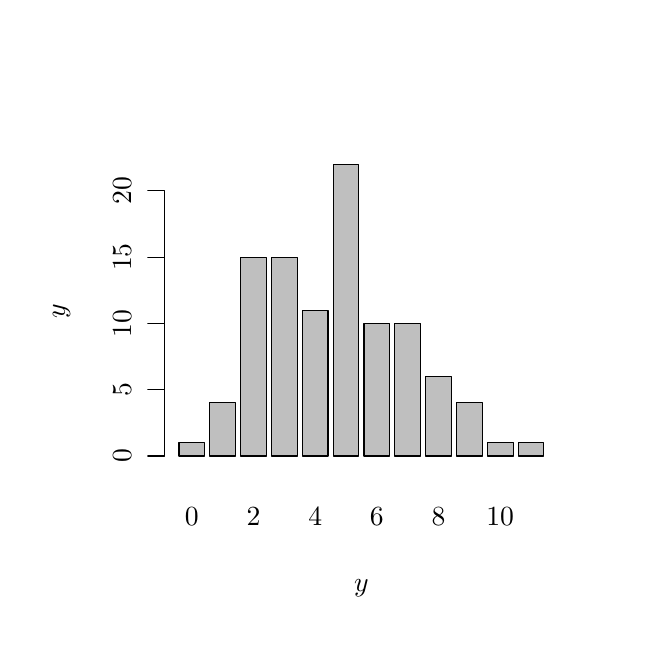
\begin{tikzpicture}[x=1pt,y=1pt]
\draw[color=white,opacity=0] (0,0) rectangle (216.81,216.81);
\begin{scope}
\path[clip] (  0.00,  0.00) rectangle (216.81,216.81);
\definecolor[named]{drawColor}{rgb}{0.88,0.97,0.36}
\definecolor[named]{drawColor}{rgb}{0.00,0.00,0.00}
\definecolor[named]{fillColor}{rgb}{0.75,0.75,0.75}

\draw[color=drawColor,line cap=round,line join=round,fill=fillColor,] ( 54.47, 62.25) rectangle ( 63.76, 67.04);

\draw[color=drawColor,line cap=round,line join=round,fill=fillColor,] ( 65.62, 62.25) rectangle ( 74.90, 81.41);

\draw[color=drawColor,line cap=round,line join=round,fill=fillColor,] ( 76.76, 62.25) rectangle ( 86.05,134.09);

\draw[color=drawColor,line cap=round,line join=round,fill=fillColor,] ( 87.90, 62.25) rectangle ( 97.19,134.09);

\draw[color=drawColor,line cap=round,line join=round,fill=fillColor,] ( 99.05, 62.25) rectangle (108.33,114.93);

\draw[color=drawColor,line cap=round,line join=round,fill=fillColor,] (110.19, 62.25) rectangle (119.48,167.61);

\draw[color=drawColor,line cap=round,line join=round,fill=fillColor,] (121.33, 62.25) rectangle (130.62,110.14);

\draw[color=drawColor,line cap=round,line join=round,fill=fillColor,] (132.48, 62.25) rectangle (141.76,110.14);

\draw[color=drawColor,line cap=round,line join=round,fill=fillColor,] (143.62, 62.25) rectangle (152.91, 90.99);

\draw[color=drawColor,line cap=round,line join=round,fill=fillColor,] (154.76, 62.25) rectangle (164.05, 81.41);

\draw[color=drawColor,line cap=round,line join=round,fill=fillColor,] (165.91, 62.25) rectangle (175.19, 67.04);

\draw[color=drawColor,line cap=round,line join=round,fill=fillColor,] (177.05, 62.25) rectangle (186.34, 67.04);
\end{scope}
\begin{scope}
\path[clip] (  0.00,  0.00) rectangle (216.81,216.81);
\definecolor[named]{drawColor}{rgb}{0.88,0.97,0.36}
\definecolor[named]{drawColor}{rgb}{0.00,0.00,0.00}

\node[color=drawColor,anchor=base,inner sep=0pt, outer sep=0pt, scale=  1.00] at ( 59.12, 37.20) {0%
};

\node[color=drawColor,anchor=base,inner sep=0pt, outer sep=0pt, scale=  1.00] at ( 81.40, 37.20) {2%
};

\node[color=drawColor,anchor=base,inner sep=0pt, outer sep=0pt, scale=  1.00] at (103.69, 37.20) {4%
};

\node[color=drawColor,anchor=base,inner sep=0pt, outer sep=0pt, scale=  1.00] at (125.98, 37.20) {6%
};

\node[color=drawColor,anchor=base,inner sep=0pt, outer sep=0pt, scale=  1.00] at (148.26, 37.20) {8%
};

\node[color=drawColor,anchor=base,inner sep=0pt, outer sep=0pt, scale=  1.00] at (170.55, 37.20) {10%
};
\end{scope}
\begin{scope}
\path[clip] (  0.00,  0.00) rectangle (216.81,216.81);
\definecolor[named]{drawColor}{rgb}{0.88,0.97,0.36}
\definecolor[named]{drawColor}{rgb}{0.00,0.00,0.00}

\node[color=drawColor,anchor=base,inner sep=0pt, outer sep=0pt, scale=  1.00] at (120.41, 13.20) {$y$
};

\node[rotate= 90.00,color=drawColor,anchor=base,inner sep=0pt, outer sep=0pt, scale=  1.00] at ( 13.20,114.41) {$\Prob{y}$
};
\end{scope}
\begin{scope}
\path[clip] (  0.00,  0.00) rectangle (216.81,216.81);
\definecolor[named]{drawColor}{rgb}{0.88,0.97,0.36}
\definecolor[named]{drawColor}{rgb}{0.00,0.00,0.00}

\draw[color=drawColor,line cap=round,line join=round,fill opacity=0.00,] ( 49.20, 62.25) -- ( 49.20,158.03);

\draw[color=drawColor,line cap=round,line join=round,fill opacity=0.00,] ( 49.20, 62.25) -- ( 43.20, 62.25);

\draw[color=drawColor,line cap=round,line join=round,fill opacity=0.00,] ( 49.20, 86.20) -- ( 43.20, 86.20);

\draw[color=drawColor,line cap=round,line join=round,fill opacity=0.00,] ( 49.20,110.14) -- ( 43.20,110.14);

\draw[color=drawColor,line cap=round,line join=round,fill opacity=0.00,] ( 49.20,134.09) -- ( 43.20,134.09);

\draw[color=drawColor,line cap=round,line join=round,fill opacity=0.00,] ( 49.20,158.03) -- ( 43.20,158.03);

\node[rotate= 90.00,color=drawColor,anchor=base,inner sep=0pt, outer sep=0pt, scale=  1.00] at ( 37.20, 62.25) {0%
};

\node[rotate= 90.00,color=drawColor,anchor=base,inner sep=0pt, outer sep=0pt, scale=  1.00] at ( 37.20, 86.20) {5%
};

\node[rotate= 90.00,color=drawColor,anchor=base,inner sep=0pt, outer sep=0pt, scale=  1.00] at ( 37.20,110.14) {10%
};

\node[rotate= 90.00,color=drawColor,anchor=base,inner sep=0pt, outer sep=0pt, scale=  1.00] at ( 37.20,134.09) {15%
};

\node[rotate= 90.00,color=drawColor,anchor=base,inner sep=0pt, outer sep=0pt, scale=  1.00] at ( 37.20,158.03) {20%
};
\end{scope}
\end{tikzpicture}
